\documentclass{article}
\usepackage[T1]{fontenc}
\usepackage{lmodern}
\usepackage{graphicx}
\usepackage{amsmath,amssymb}
\usepackage[a4paper,margin=2cm]{geometry}
\usepackage[absolute,overlay]{textpos}
\setlength{\TPHorizModule}{1mm}
\setlength{\TPVertModule}{1mm}
\usepackage[indonesian]{babel}
\usepackage{hyperref}
\setlength{\emergencystretch}{2em}
% unit: Halaman 65

\begin{document}

% === Halaman 65 (llm) ===

% (tidak ada teks dari model)

% deskripsi: Diagram logika sirkuit digital yang menunjukkan tiga register pergeseran (R1, R2, R3) dengan beberapa tap (titik pengambilan data) yang dihubungkan melalui gerbang XOR untuk menghasilkan urutan bit.
% bbox normalisasi: [0.1380, 0.1830, 0.8310, 0.8230]
\begin{textblock*}{145.53mm}(28.98mm,54.35mm)
\noindent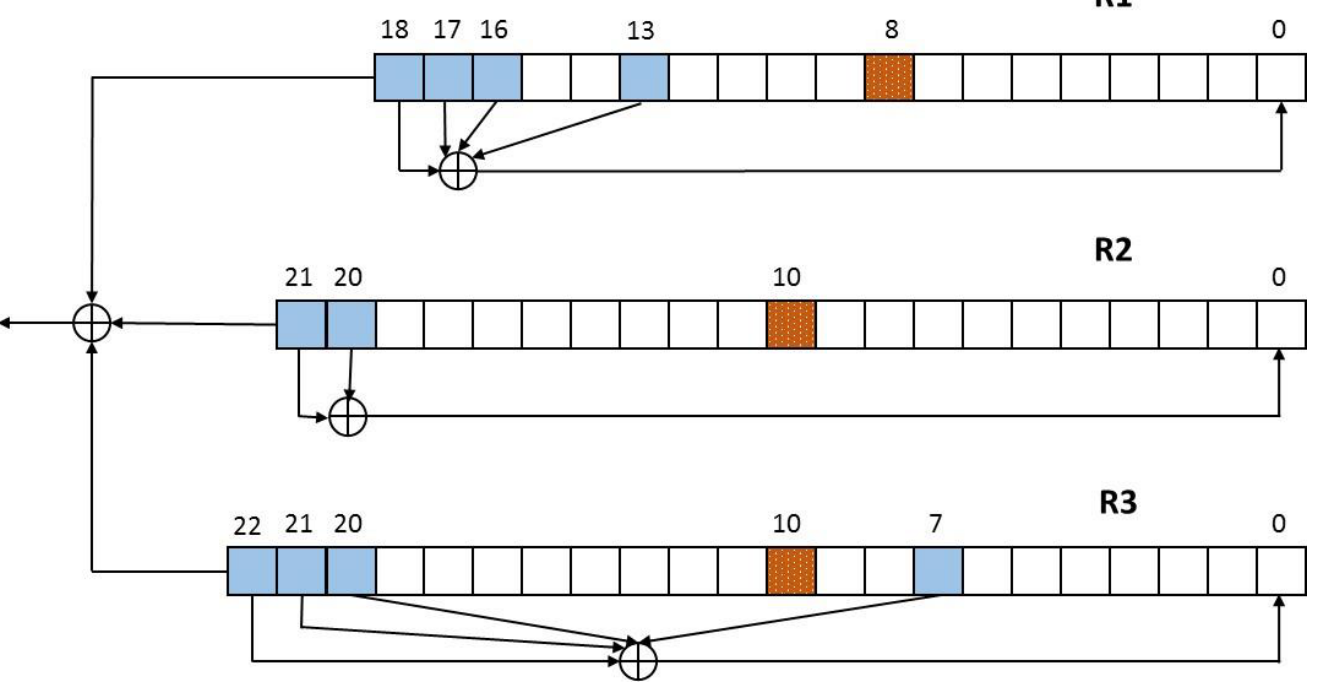
\includegraphics[width=145.53mm,height=190.08mm]{../../images/llm/page_065_img_01.png}%
\end{textblock*}

\end{document}
